\documentclass[a4paper, 10pt]{article}
\usepackage[italian]{babel}
\usepackage{kpfonts}
\usepackage[T1]{fontenc}
\usepackage[utf8]{inputenc}
\usepackage{amsmath}
\usepackage{amsfonts}
\usepackage{amsthm}
\usepackage{commath}
\usepackage{amssymb}
\usepackage{bm}
\usepackage{epigraph}
\usepackage{hyperref}
\hypersetup{
	hidelinks, 
	colorlinks = true,
	linkcolor = black
}
\usepackage{wrapfig}
\usepackage{multicol}
\usepackage{graphicx}
\usepackage{tikz}
\usetikzlibrary{arrows}
\usetikzlibrary{shapes,positioning,calc}
\usepackage{geometry}
\geometry{a4paper, left=3cm,right=3cm,top=3cm,bottom=3cm}
\usepackage{fancyhdr}
\pagestyle{fancy}
\lhead{\nouppercase{\leftmark}}
\rhead{\nouppercase{\rightmark}}
\chead{}
\lfoot{}
\cfoot{\thepage}
\rfoot{}
\renewcommand{\headrulewidth}{0.4pt}
\renewcommand{\footrulewidth}{0.4pt}

\setlength{\columnsep}{0.1cm}

\renewcommand{\vec}{\bm}
\newcommand*\diff{\mathop{}\!\mathrm{d}}
\newcommand{\numberset}{\mathbb}
\newcommand{\R}{\numberset{R}}

\title{Grafica al Calcolatore}
\author{Matteo Danzi}
\date{}

\begin{document}
	\maketitle
	
	\tableofcontents
	
	\newpage
	
	\section{Introduzione}
		\textit{Cos'è grafica al calcolatore} ? Intuitivamente è l'uso di un calcolatore per produrre un'immagine o una sequenza di immagini, non necessariamente realistica o in 3D, non necessariamente interattiva.
		
		\noindent
		Per \textbf{computer grafica}, \textbf{grafica digitale} o \textbf{grafica computerizzata} (in inglese \textbf{computer graphics}) si intende:
		\begin{itemize}
			\item Creazione immagini 2d sintetiche e animazioni
			\item Modellazione 2D, 3D, anche con comportamenti fisici
			\item Computer Aided Design
			\item Rendering delle scene, cioè creazione delle immagini simulando la
			proiezione ottica delle scene sulla camera
			\item Animazione
			\item Interfacce grafiche dei computer
			\item Realtà virtuale
			\item Enhancement video televisivo
			\item Visualizzazione scientifica e dell'informazione
		\end{itemize}
		
	\subsection{Storia}
		Nasce con i primi display per calcolatori. 
		
		\noindent
		Nel 1960 William Fetter introduce il termine \textbf{Computer Graphics} per descrivere la ricerca che stava conducendo alla Boeing. Questa ricerca ha portato alla realizzazione di un modello 3D del corpo umano per progettare la carlinga degli aerei. Nasce quindi l'idea della modellazione 3D che rappresenta una parte rilevante della moderna CG. 
		
		\noindent
		Nel 1963 assistiamo alla nascita della \textbf{Computer Grafica interattiva}: sistema sketchpad di Ivan Sutherland. In questo caso si tratta della prima \textbf{interfaccia grafica} interattiva.
		
		\noindent
		Negli anni '60 inoltre nascono i primi terminali grafici e i primi giochi, si impara quindi a disegnare sullo schermo 2D. Nel 1961 Steve Russell at MIT crea il primo video game, Spacewar.
		
		\noindent
		Negli anni '70 nascono le moderne \textbf{interfacce grafiche interattive} dei computer (WIMP - \textit{Window, Icon, Menu and Pointing device}). La grafica interattiva, in questo caso 2D diventa parte integrante del sistema di interazione	uomo-macchina.
		
		\noindent
		Nel 1972 nasce il videogioco Pong (Atari). Anche oggi una delle maggiori applicazioni della	grafica interattiva è nel mondo dei \textbf{videogiochi}.
		
		\noindent
		Negli anni settanta nascono	gli algoritmi per creare immagini da modelli 3D	(\textbf{rendering}).
		Nel 1972 Catmull (Univ. Utah) crea la prima animazione di grafica 3D. Si tratta di un modello della sua mano formato da 350 poligoni. Catmull diventerà un cofondatore della \textit{Pixar} (oggi presidente).
		
		\noindent
		Gli algoritmi per creare linee raster, riempire poligoni, proiettare oggetti 3D su telecamere virtuali vengono via via sviluppati negli anni '60-70-80. Questi argomenti sono il cuore della grafica 3D e di questo corso.
		
		\noindent
		Si creano standard e implementazioni di sistemi grafici e si arriva alla situazione attuale:
		\begin{itemize}
			\item 1992 Silicon Graphics crea lo standard \textbf{OpenGL}
			\item 1995 Microsoft rilascia Direct 3D
		\end{itemize}
		La grafica ha pesantemente condizionato lo sviluppo	dell'hardware e l'architettura dei moderni calcolatori (e tablet, smartphone, ...)
		
		\noindent
		Le operazioni grafiche vengono implementate su hardware	specifico
		Inizialmente grafica raster calcolata su CPU, poi (doppio) buffer per mantenere le immagini (doppio perché il calcolo può essere lento rispetto al refresh dello schermo)
		Nel 1985 esce il Commodore Amiga, uno dei primi home computer con una GPU (Graphical Processing Unit), nel 1987 il primo PC Ibm con operazioni 2D hardware.
		
		\noindent
		Nel 1995 escono le prime schede video per PC con pipeline grafica 3D (S3 Virge), nel 1999 Nvidia GeForce 256 la prima scheda con transform \& lightning engine.
		
		
	\subsection{Applicazioni}
		\begin{itemize}
			\item \textbf{Modellazione 3D}: prototipazione e stampa 3D, digital manufacturing
			\item \textbf{Grafica non interattiva}: cinema digitale, grafica pubblicitaria, ecc.
			\item \textbf{Grafica interattiva}:
				\begin{itemize}
					\item \textit{Visualizzazione scientifica}: uso della grafica (2D-3D) per comunicare efficacemente informazione di misure o simulazioni
					\item \textit{Visualizzazione dell'informazione}: creazione di modelli "mentali" utili per rappresentare nello spazio dati	astratti
					\item Realtà virtuale o aumentata e interazione uomo macchina
					\item Interfacce naturali per comunicare con i computer o simulare attività reali
					\item Simulatori, Videogiochi
				\end{itemize}
		\end{itemize}
		\noindent
		Grafica è quindi una \textit{disciplina che studia le tecniche e gli algoritmi per la
		rappresentazione visuale di informazioni numeriche prodotte o
		semplicemente elaborate dai computer} (da Scateni e al.).
		
		\noindent
		È quindi legata a molte altre discipline.
		
		\begin{center}
			\begin{tikzpicture}[baseline=1.5cm]
			\node[draw, ellipse, align=center] (centre) at (0,0) {\Huge Computer\\ \Huge Graphics};
			\node[draw, ellipse, align=center, fill=white] (a) at ($ (centre.west) -(1,0) $) {Image\\ processing};
			\node[draw, ellipse, align=center, fill=white] (b) at ($ (centre.west) -(0,1.5) $) {Geometria\\ Computazionale};
			\node[draw, ellipse, align=center, fill=white] (c) at ($ (centre.south) -(-0.5,0.5) $) {Pattern\\ recognition};
			\node[draw, ellipse, align=center, fill=white] (d) at ($ (centre.east) -(0,1) $) {Computer\\ Vision};
			\node[draw, ellipse, align=center, fill=white] (a) at ($ (centre.east) +(0.25,0.5) $) {Fisica};
		\end{tikzpicture}
		\end{center}
		
	\subsection{Computer Graphics vs Computer Vision}
		In senso generale la grafica è il meccanismo opposto dell'\textbf{image understanding} o della \textbf{computer vision}.
		
		\noindent
		Nel primo caso si passa da immagini a parametri, a interpretazione. Nel secondo si crea un'immagine da un input parametrico. Quindi sono grafica tutti i sistemi informatici che creano
		e usano immagini sintetiche.
		
	\subsection{Visual Computing}
		Oggi vista la convergenza dei due domini si parla spesso in
		generale di \textit{ visual computing}.
		
		\noindent
		Visual computing is a generic term for all computer science
		disciplines handling with images and 3D models, i.e. computer
		graphics, image processing, visualization, computer vision,
		virtual and augmented reality, video processing, but also
		includes aspects of pattern recognition, human computer
		interaction, machine learning and digital libraries. The core
		challenges are the acquisition, processing, analysis and
		rendering of visual information (mainly images and video).
		Application areas include industrial quality control, medical
		image processing and visualization, surveying, robotics,
		multimedia systems, virtual heritage, special effects in movies
		and television, and computer games.
		
		\newpage
		
	\section{Applicazioni}
		Se lo scopo della grafica al calcolatore è quello di riprodurre un
		grafico, quel che dovrà fare il nostro software è preparare i
		valori di output da passare al nostro display.
		
		\noindent
		Il display (output) può essere differente a seconda
		dell'applicazione. In generale sarà un \textbf{display raster} come un monitor, che riproduce una matrice di punti su cui è codificata una terna di valori di colore RGB
		Sono dominio della grafica le applicazioni che
		\begin{itemize}
			\item Preparano file per la stampa 2D (grafica vettoriale)
			\item Stampa 3D
			\item Display innovativi (ad esempio stereo, volumetrici)
		\end{itemize}
		Possiamo rappresentare la grafica in un dato digitale in due modi:
		\begin{enumerate}
			\item \textbf{Vettoriale} : utilizzando primitive di disegno
			\item \textbf{Raster}: utilizzando una griglia di valori da riprodurre sul monitor
		\end{enumerate}
		
	\subsection{Grafica vettoriale}
		La rappresentazione grafica vettoriale compone le immagini come un \textit{\textbf{insieme di primitive di disegno}} come ad esempio \textit{Linee}, \textit{Curve}, \textit{Aree}.
		
		\noindent
		Queste possono essere descritte con \textbf{funzioni parametriche} e \textbf{coordinate di punti}.
		
		\noindent
		Dove vengono applicate:
		\begin{itemize}
			\item Disegno su display vettoriali.
			\item Plotter.
			\item Rappresentazione per la stampa, necessita di conversione a raster di
			solito effettuata dalla stampante.
			\item Rappresentazione interna nei calcolatori di forme grafiche che
			devono essere rappresentate a differente livello di precisione (Es. caratteri di stampa che facciamo grandi o piccoli, ecc.).
		\end{itemize}
		
		\noindent
		Vantaggi:
		\begin{itemize}
			\item I dati sono espressi in una forma direttamente comprensibile ad un
			essere umano (es. lo standard SVG);
			\item Compattezza di codifica rispetto all'equivalente raster;
			\item Possibilità di ingrandire l'immagine arbitrariamente, senza che si
			verifichi una perdita di risoluzione dell'immagine stessa.
		\end{itemize}
		Limiti: per la rappresentazione sulla maggior parte dei display occorre poi
		convertire a raster.
		
		\begin{figure}[h!]
			
\includegraphics[scale=0.4]{tiger1.png}
			\hspace*{0.4cm}
			
\includegraphics[scale=0.4]{tiger.png}
			\hspace*{0.4cm}
			
\includegraphics[scale=0.4]{tiger1.png}
			\hspace*{0.4cm}
			
\includegraphics[scale=0.4]{tiger2.png}
			\caption{Differenza di scalatura tra raster(sx) e vettoriale(dx) }
		\end{figure}
		
		
		\newpage
		
	\subsection{Immagini Raster o bitmap}
		Le immagini digitali cui siamo abituati con i monitor immagini
		\textbf{raster} e consistono di una matrice di elementi denominati
		\textbf{pixel} dove ogni cella della matrice rappresenta un colore in rgb.
		
		\noindent
		Il nostro software scriverà quindi un \textit{frame buffer}: memoria
		contenente l’immagine, array di valori per i pixel, che viene
		modificato direttamente dal programma di grafica video
		controller il quale legge il frame buffer e costruisce l’immagine
		sul display.
		
		\begin{figure}[h!]
			\centering
			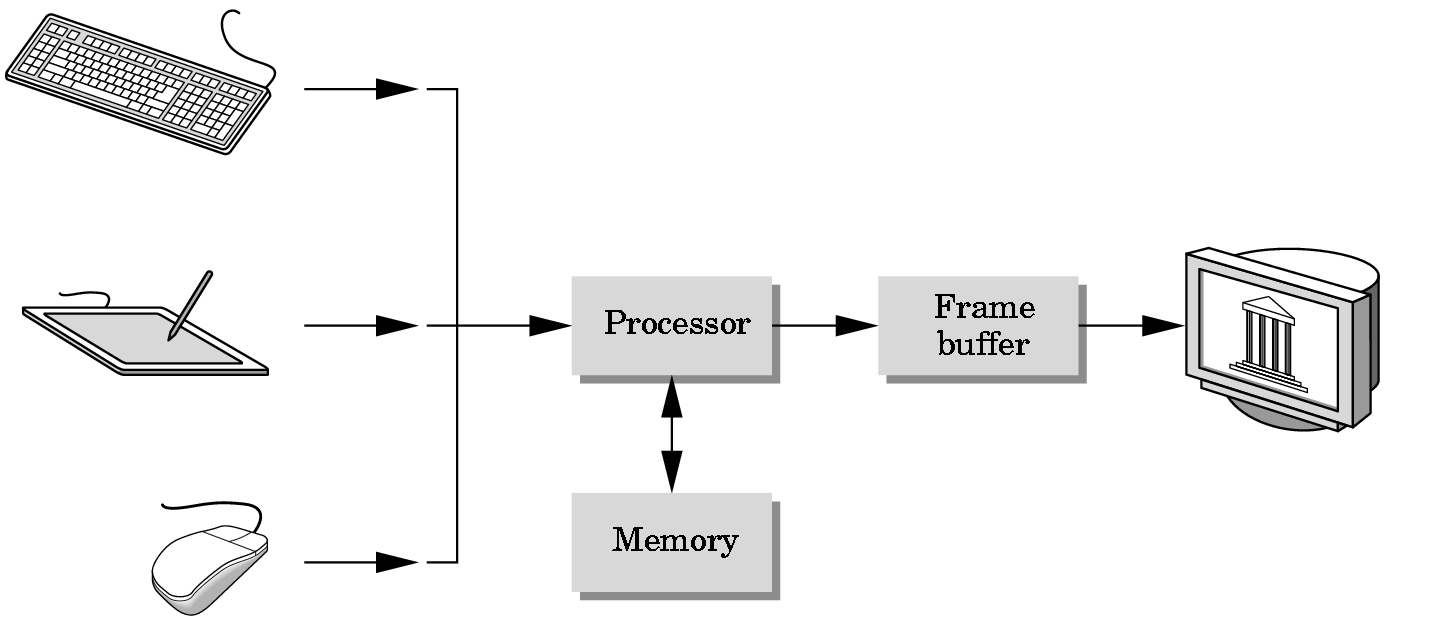
\includegraphics[scale=0.2]{img.png}
		\end{figure}
		\begin{center}
			\begin{tikzpicture}[>=latex, scale=.6]
			\draw (3,-3) -- (4,-2) -- (4,0) -- (2,0) -- (1,-1) ;
			\draw (3,-1) -- (4,0);
			\draw  (1,-1) rectangle (3,-3);
			\node [below] at (2,-3.5) {model};
			\draw[->] (4.5,-2) -- node[above, align=center] {graphics\\software} (6.5,-2);
			\foreach \i in {0.0, -0.5,..., -3}{
				\draw[fill=black] (7.5, \i) rectangle (7.1, \i-0.4);
				\foreach \x in {7.5,8,...,10.5}{
					\draw (\x, \i) rectangle (\x-0.4, \i-0.4);
					\draw[fill=black] (\x, -2) rectangle (\x-0.4, -2.4);
				}
			}
			
			
			\node [below] at (9,-3.5) {frame buffer};
			\draw[->] (11,-2) -- node[above, align=center] {graphics\\hardware} (13,-2);
			\draw (14,0) rectangle (18,-3) ;
			\node [below] at (16,-3.5) {monitor screen};
			\draw (18, -3) -- (19, -2) -- (19, 1) -- (15, 1) -- (14, 0);
			\draw (18,0) -- (19,1);
			\draw[fill=black] (14.5,-0.5) rectangle (17.5,-2.5);
			\draw[fill=white] (16.5,-2.5) -- (17,-2) -- (17,-1) -- (16,-1) -- (15.5,-1.5);
			\draw[fill=white] (15.5,-1.5) rectangle (16.5,-2.5);
			\draw (17,-1) -- (16.5,-1.5);
			
		\end{tikzpicture}
		\end{center}
		
		\noindent
		Le immagini raster sono \textbf{matrici} che contengono valori che rappresentano il colore
		nella casella corrispondente agli indici con valori discretizzati.
		
		\noindent
		Di solito ci sono componenti di colore: i monitor generano il colore
		con sovrapposizione di luce rossa, verde e blu (Perché?)
		
		\noindent
		Caratteristiche principali (non le uniche): 
		\begin{itemize}
			\item \textbf{risoluzione} (dimensioni della matrice di pixel)
			\item \textbf{profondità di colore} (bit di memoria per pixel).
		\end{itemize}
		8-bit significano 256 colori, mentre 24-bit (o truecolor)
		rappresentano all’incirca 32 milioni di colori
		
		\noindent
		\textbf{Nota}: è la rappresentazione di uscita tipica di quasi tutti i
		display odierni, ma non è ovviamente l'unica possibile
		\begin{itemize}
			\item Es.: display vettoriali: riproducono disegni
			\item Il formato digitale creato internamente deve ovviamente
			corrispondere alla capacità del display scelto di riprodurlo
		\end{itemize}
		
		Nel processo di rasterizzazione delle immagini vettoriali la qualità della
		conversione dipende	dalla risoluzione dell'immagine originale (numero di punti o punti per pollice).
		
		\noindent
		Un effetto possibile può essere la scalettatura: effetto dell'\textbf{aliasing} delle alte frequenze.
		Si può ridurre tale effetto sfumando la luminosità e facendo quindi \textit{antialiasing}.
		
		\begin{figure}[h!]
			\centering
			
\includegraphics[scale=0.2]{alias.png}
			\hspace*{0.4cm}
			
\includegraphics[scale=0.2]{alias1.png}
			\hspace*{0.4cm}
			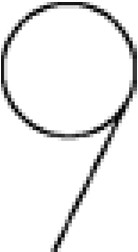
\includegraphics[scale=0.2]{alias2.png}
			\hspace*{0.4cm}
			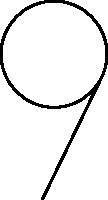
\includegraphics[scale=0.25]{alias3.png}
		\end{figure}
		
	\subsection{Aliasing}
		L'aliasing accade perché l'immagine è il campionamento di un segnale "continuo" che rappresenterebbe il dato misurabile.
		\[
			I(i, j) = I(i\Delta x, j\Delta y) = \iint F (x, y)\delta (x - i\Delta x)\delta (y - i\Delta y)
		\]
		
		\begin{center}
			\begin{tikzpicture}[>=latex, scale=0.5]
			\foreach \x in {0, 1, ..., 5}{
				\foreach \i in {0, -1, ..., -5}{
					\fill (\x,\i) circle (4pt);
				}
			}
			\draw[<->] (-0.5,-5) -- node[left] {$ \Delta y$} (-0.5,-4);
			\draw[<->] (0,-5.5) -- node[below] {$ \Delta x$} (1,-5.5);
		\end{tikzpicture}
		\end{center}
		
		Per il \textit{teorema di Shannon/Nyqvist} del campionamento, non si
		può ricostruire esattamente il segnale originale se la frequenza
		del segnale è superiore alla metà della frequenza di
		campionamento.
		
		\[
			v_{cx} = \dfrac{1}{\delta x} \geq 2v_{x max} \qquad 
			v_{cy} = \dfrac{1}{\delta y} \geq 2v_{y max} 
		\]
		
		Dove ci sono discontinuità del colore, ci sono componenti a
		frequenza alta, si creano artefatti. I filtri che fanno antialiasing attenuano le alte frequenze.
		
		
	\subsection{Caratteristiche Immagini raster}
		Le principali caratteristiche delle immagini raster sono:
		\begin{itemize}
			\item \underline{Risoluzione} (numero di righe e colonne matrice)
			\item \underline{Range dinamico}: rapporto tra minima differenza misurabile o
			rappresentabile e range di variabilità del segnale (luminosità). Corrisponde al numero di bit con cui codifichiamo il valore. Tipicamente 8 bit ma si può andare oltre:
			\begin{itemize}
				\item Immagini HDR
				\item Immagini mediche
				\item Dato che l'occhio umano non distingue così tante sfumature, lo
				scopo è di poter creare da esse rendering diversi che possano dare
				differenti effetti o informazioni
			\end{itemize}
			Il valore codificato dovrebbe corrispondere alla luminosità del
			punto generata dal monitor o acquisita dal sensore, ma la cosa
			è un po' più complicata a causa della \textbf{non-linearità della
			percezione umana}.
		\end{itemize}
		Insomma quello che c'è nel file non è quello che vediamo. Il rendering ed il dispositivo determinano la visualizzazione. E poi c'è il fattore legato alla percezione umana. 
		Ad esempio: immagini ad alto range dinamico (HDR) (Mantiuk et al 2005)
		
		\noindent
		La percezione umana amplifica le differenze del range dinamico ai bassi livelli. Macchine fotografiche e monitor applicano correzioni (gamma correction)
		
		\subsubsection{Colore}
			Le immagini raster da inviare ai display sono in genere a colori,
			per simulare il modo in cui vediamo il mondo (a colori).
			La rappresentazione del colore è generalmente una \textit{terna di
			valori RGB}.
			Per la riproduzione corrispondono alle intensità emesse da tre
			emettitori di luce a tre frequenze determinate (rosso, verde,
			blu) che danno origine in corrispondenza a un certo colore
			percepito dall'utente.
			
			\noindent
			\textit{Ma cosa significa questo?}
			
			\noindent
			Nei monitor si generano i colori nei punti della griglia per
			sintesi additiva: si mescolano due o più fasci luminosi di
			diversa.
			
			\noindent
			Nella stampa per sintesi sottrattiva: Due o più inchiostri
			sovrapposti assorbono diverse frequenze e cambiano la luce
			diretta all'occhio.
			
			\noindent
			Non tutti i colori possono essere generati in mescolanza
			additiva o sottrattiva di tre colori primari
			La scelta di \textbf{Rosso Verde Blu} come \textit{primari additivi} e \textbf{Giallo,
			Magenta e Cyan (e nero)} \textit{sottrattivi} cerca di massimizzare i
			colori rappresentabili
		
			\begin{wrapfloat}{figure}{I}{0pt}
				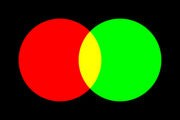
\includegraphics[width=0.3\textwidth]{colors}
			\end{wrapfloat}
		
			\noindent
			L'uso delle 3 componenti di colore RGB è
			convenzionale e deriva dalla fisiologia della
			visione, che mostra che con 3 colori base si
			possono approssimativamente riprodurre i
			colori del mondo reale.
			
			\noindent
			I colori visibili però derivano invece da una
			variazione continua di lunghezza d'onda delle
			radiazioni elettromagnetiche in un intervallo
			percettibile di valori circa 370-730 nm.
			
			\noindent
			\textbf{Percezione del colore}: nella retina ci sono 3 tipi di coni, che
			hanno differenti sensitività a diverse frequenze S,M,L
			Possiamo fare il matching delle frequenze con la risposta dei
			recettori.
			
			\bigskip
			
			Il "colore" percepito è dato da 3 grandezze scalari, funzione
			dello spettro della luce incidente.
			La corrispondenza non è iniettiva. Spettri diversi possono
			corrispondere allo stesso colore percepito: metamerismo
			Conseguenza: Per riprodurre un colore, non è necessario
			riprodurre lo spettro. È sufficiente che le risposte L, M, S dei
			coni siano uguali.
			Può cambiare in funzione dell'illuminazione.
			
			\noindent
			\textbf{Metamerismo}: consiste nella possibilità di ottenere un effetto ottico tale che l'occhio percepisca la stessa sensazione di colore in presenza di luce con distribuzione spettrale diversa dal colore puro in questione.
			Si tratta di un'illusione ottica basata sulla natura dell'interpretazione del colore da parte dell'occhio umano, è possibile creare la sensazione di un colore "puro", formato, selezionando la sola lunghezza d'onda che genera quella determinata sensazione di colore miscelando a dovere più lunghezze d'onda differenti, un esempio è il bianco di una lampada fluorescente formato da spettri non uniformi, in questo caso la temperatura di colore che si trova sulle confezioni è la temperatura a cui deve essere un corpo nero perché l'occhio umano percepisca la stessa sensazione di colore.
			Il fenomeno si ha quando colori che appaiono all'occhio identici sotto una certa luce, mostrano tonalità differenti se illuminati con una luce diversa. In sostanza c'è metamerismo quando due colori si equivalgono sotto una fonte di luce, ma risultano differenti ad altre esposizioni.
			
		\subsubsection{Legge di Grassman}
			L'uomo è in grado di fare match di colori mischiando 3 (o
			più) colori detti primari. Se la luce test $ T $ ha un certo colore:
			\[
				T = aP1 + bP2 + cP3
			\]
			il match si verifica lineare.
			
		\subsubsection{Funzioni di Matching}
			Data una terna di colori di base possiamo studiare il matching
			dei colori sugli osservatori in funzione della frequenza.
			Componenti colore CIERGB ricavate dall'integrale delle
			frequenze dello stimolo su tutto il range.
			
			\begin{align*}
				L &= \int \Phi (\lambda) L (\lambda) \diff\lambda \\
				M &= \int \Phi (\lambda) M (\lambda) \diff\lambda \\
				S &= \int \Phi (\lambda) S (\lambda) \diff\lambda 				
			\end{align*}
			
			Rappresentazione con matrice:
			\[
			C =
			\begin{pmatrix}
			\overline{r} (\lambda_1) & \dots & \overline{r}(\lambda_N) \\
			\overline{g} (\lambda_1) & \dots & \overline{g}(\lambda_N) \\
			\overline{b} (\lambda_1) & \dots & \overline{b}(\lambda_N) 
			\end{pmatrix}
			\]
			\[
			\Phi =
			\begin{pmatrix}
			\phi(\lambda_1)\\
			\vdots \\
			\phi (\lambda_N) 
			\end{pmatrix}
			\]
			
	\section{Schema di un'applicazione grafica}
		Vi è una descrizione di qualche tipo (procedurale o meno) del
		mondo che deve essere rappresentato. La produzione di tale
		descrizione (modello) prende il nome di \textbf{modellazione}.
		
		\noindent
		Da tale descrizione si ottiene una immagine visualizzabile da
		un display tale processo è chiamato globalmente \textbf{rendering}.
		
		\noindent
		La sequenza di procedure ed algoritmi che implementano il
		rendering prende il nome di \textbf{pipeline grafica}.
		
		\noindent
		Se l'applicazione è interattiva, il disegno dev'essere riprodotto
		in real time mentre l'utente interagisce con la scena mediante
		dei dispositivi.
			
	\subsection{Modello della scena}
		Nelle applicazioni 2D può essere un disegno da riprodurre sul
		display a meno di una trasformazione geometrica e mappatura
		sui pixel.
		Nelle applicazioni 3D di cui ci interesseremo sarà invece un
		vero e proprio modello del "mondo" che vogliamo vedere (e
		con cui vogliamo interagire) e l'immagine sarà generata
		simulando il processo di acquisizione di immagini di una
		telecamera "virtuale".
		
		\noindent
		Dati gli oggetti della scena, quindi dovremo "simulare" la geometria
		e la fisica della formazione delle immagini (luce, colore)
		
	\subsection{Rendering della scena}
		Il passaggio dalla rappresentazione all'immagine si definisce
		\textit{rendering}.
		
		\noindent
		Comprende tutti gli algoritmi per creare l'immagine per il
		display, che supporremo voglia un'immagine raster.
		
		\noindent
		Quindi se partiamo da una \textbf{rappresentazione 2D} (grafica
		vettoriale) il rendering consiste in:
		\begin{enumerate}
			\item Trasformazione delle primitive in rappresentazioni di colore sui pixel
			(rasterizzazione)
			\item Eventuale modifica interattiva del disegno
		\end{enumerate}
		Se partiamo da una \textbf{rappresentazione di scena 3D} il rendering consiste in:
		\begin{enumerate}
			\item Proiezione della scena sul piano immagine della telecamera virtuale
			\item Trasformazione della scena proiettata in rappresentazioni di colore
			sui pixel (rasterizzazione)
			\item Eventuale interazione con la scena e conseguenteupdate del
			rendering
		\end{enumerate}
		
		Il rendering comprende molti calcoli da svolgere, la \textbf{complessità} dipende dall'applicazione di interesse:
		\begin{itemize}
			\item Applicazioni interattive, real-time:
			\begin{itemize}
				\item Frame rate alto (>10 fps)
				\item Tempo di rendering del singolo frame prefissato
				\item Si può/deve sacrificare la qualità per garantire l’interattività
			\end{itemize}
			\item Applicazioni non interattive (computer animation, grafica
			pubblicitaria)
			\begin{itemize}
				\item l'obiettivo primario: massima qualità delle immagini di sintesi
				\item Non si hanno vincoli sul tempo di generazione del singolo frame
				\item Animazioni calcolate frame by frame da PC cluster, ricomposte
				successivamente nella successione temporale corretta
			\end{itemize}
		\end{itemize}
		
		Come si implementa la fase di rendering?
		\begin{itemize}
			\item Applicazioni interattive: si avvalgono pesantemente delle moderne schede grafiche (HW
				dedicato al processing di dati 3D)
			\item Applicazioni non interattive: fanno uso di ambienti di rendering più sofisticati e flessibili (ad es. RenderMan), spesso eseguiti SW su cluster di PC
		\end{itemize}
		
	\section{Modellare lo spazio}
		Richiamiamo le nozioni basilari di geometria per modellare lo
		spazio e gli oggetti:
		\begin{itemize}
			\item \textbf{Scalari}: unidimensionali, possono rappresentare grandezze fisiche
			con numeri
			\item \textbf{Punti}: rappresentano una posizione nello spazio
			\item \textbf{Vettori}: rappresentano le direzioni o le distanze tra punti in 2D o 3D
		\end{itemize}
		Per definire una posizione nello spazio dobbiamo introdurre un
		sistema di riferimento con un punto fisso detto origine e una
		terna di direzioni ortogonali
		
		\subsection{Scalari}
			Gli scalari S costituiscono un corpo (tipicamente useremo IR)
			con due operazioni, somma e moltiplicazione, che soddisfano
			le seguenti relazioni:
			
			\begin{multicols}{2}
				\begin{center}
					$ \forall \alpha,\beta,\gamma \in S $
				
				\noindent
				\textbf{Commutatività}
				\begin{align*}
					\alpha + \beta &= \beta + \alpha \\
					\alpha \beta &= \beta\alpha
				\end{align*}
				
				\textbf{Associatività}
				\begin{align*}
					\alpha + (\beta + \gamma) &= (\beta + \alpha) + \gamma \\
					(\alpha\beta)\gamma &= \alpha(\beta\gamma)
 				\end{align*}
				
				\textbf{Distribuzione}
				\[
					\alpha(\beta + \gamma) = \alpha\beta + \alpha\gamma
				\]
				
				\columnbreak
				
				\textbf{Elementi neutri}
				\begin{align*}
					\exists 0 \in S \: &: \: \forall \alpha \in S \quad \alpha + 0 = \alpha \\
					\exists 1 \in S \: &: \: \forall \alpha \in S \quad \alpha 1 = \alpha 
				\end{align*}
				
				\textbf{Elementi inversi}
				\begin{align*}
				\forall \alpha \in S \quad & \exists (-\alpha) \in S \: : \: \alpha + 0 = \alpha \\
				\forall \alpha \in S \quad & \exists \alpha^{-1} \in S \: : \: \alpha\alpha^{-1} = 1 
				\end{align*}
				\end{center}
			\end{multicols}
			
		\subsection{Vettori}
			I vettori costituiscono un \textbf{gruppo
			abeliano} (commutativo) $ V $ in cui e
			definito il \textbf{prodotto di un vettore
			per uno scalare}.
		
			\begin{multicols}{3}
				\begin{center}
				\textbf{Chiusura}
				\begin{align*}
					\vec{u} + \vec{v} \in V &\quad \forall \vec{u}\vec{v} \in V \\
					\alpha \vec{v} \in V &\quad \forall \alpha \in S \: \vec{v} \in V
				\end{align*}
				\columnbreak
				
				\textbf{Proprietà Algebriche}
				\begin{align*}
					\vec{u} + \vec{v} &= \vec{v} + \vec{u} \\
					\vec{u} + (\vec{v} + \vec{w}) &=  (\vec{u} + \vec{v}) + \vec{w} \\
					\alpha(\vec{u} + \vec{v}) &= \alpha\vec{u} + \alpha\vec{v} \\
					(\alpha + \beta)\vec{u} &= \alpha\vec{u} + \beta\vec{u}
				\end{align*}
				
				\begin{align*}
					\exists 0 &\in V \: : \: \forall \vec{u} \in V \quad \vec{u} + 0 = \vec{u} \\
					\forall \vec{u} &\in V \: \: \exists(-\vec{u}) \in V \: : \: \vec{u} + (-\vec{u}) = \vec{0}
				\end{align*}
			\end{center}
			\end{multicols}
		
			La definizione è totalmente
			astratta, ma per semplicità
			conviene considerare due utili
			esempi di spazi vettoriali lineari: Geometrico e Algebrico.
			
			\noindent
			Un esempio concreto e dato
			dai segmenti orientati liberi,
			ovvero senza un punto di
			applicazione specificato
			Il prodotto con uno scalare
			(numeri reali) cambia la
			lunghezza del vettore.
			La somma di due vettori e
			data dalla regola del
			parallelogramma.
			
			\begin{tikzpicture}[>=latex, baseline=0.5cm]
				\draw[thick, ->] (0,-2) -- (2,0) node[midway, left] {$ \vec{v} $};
				\draw[thick, ->] (0,-3) -- (3,0) node[midway, left] {$ 2\vec{v} $};
			\end{tikzpicture}
			\hspace*{0.5cm}
			\begin{tikzpicture}[>=latex, baseline=0.5cm]
				\draw[thick, <-] (0,-2) -- (2,0) node[midway, left] {$ -\vec{v} $};
				\draw[thick, ->] (4,-2) -- (6,0) node[midway, left] {$ \vec{v} + \vec{u} $};
				\draw[thick, ->] (4,-2) -- (5.5,-1.5) node[midway, below] {$ \vec{v}$};
				\draw[thick, ->] (5.5,-1.5) -- (6,0) node[midway, right] {$ \vec{u} $};
			\end{tikzpicture}
			
			\vspace*{0.5cm}
			
			\noindent
			Un altro esempio è dato dall'insieme delle n-ple ordinate di $ \R^n $.
			\[
				\vec{v} = (\beta_1, \dots, \beta_n) \quad \beta_i \in \R \forall i
			\]
			Il prodotto per uno scalare e la somma di due vettori sono
			definiti in modo del tutto naturale:
			\begin{align*}
				(\alpha_1, \dots, \alpha_n) + (\beta_1, \dots, \beta_n) &= 
				(\alpha_1 + \beta_1, \dots, \alpha_n + \beta_n) \\
				\alpha(\beta_1, \dots, \beta_n) &= (\alpha\beta_1, \dots, \alpha\beta_n)
			\end{align*}
			E' facile vedere qual è l'elemento neutro e qual è l'inverso di un
			vettore.
			
		\subsubsection{Indipendenza lineare}
			Dati n vettori non nulli, si dicono \textbf{linearmente indipendenti} se
			qualsiasi loro combinazione lineare a coefficienti non tutti nulli
			è diversa dal vettore nullo.
			\[
				\alpha_1\vec{v}_1 + \dots + \alpha_n \vec{v}_n = \vec{0} \: \Leftrightarrow \: \alpha_i = 0 \forall i
			\]
			Si dice \textbf{dimensione} di uno spazio vettoriale il massimo numero
			di vettori linearmente indipendenti.
			
			\noindent
			In uno spazio vettoriale a dimensione n, un insieme di n vettori
			linearmente indipendenti si dice una \textbf{base} per lo spazio.
			Ogni vettore può essere scritto come combinazione lineare dei
			vettori di una base.
		\subsubsection{Rappresentazione in componenti}
			Fissata quindi una \textbf{base in uno spazio vettoriale}, ad ogni
			vettore corrisponde una n-pla di scalari, ovvero i coefficienti
			dello sviluppo lineare del vettore nei vettori di base; tali scalari
			sono le componenti del vettore rispetto alla base data.
			
			\noindent
			In genere il corpo è dato dai reali; abbiamo quindi ottenuto la
			rappresentazione concreta vista prima di uno spazio vettoriale
			astratto come insieme di n-ple di $ \R^n $.
			Tale rappresentazione dipende dalla base scelta.
			
		\subsection{Punti}
			I vettori non rappresentano punti nello spazio, ma solo
			spostamenti. Per poter introdurre il concetto di \textbf{posizione} si
			deve passare agli \textbf{spazi affini} che sono degli spazi vettoriali a
			cui si aggiunge il concetto astratto di punto.
			
			\noindent
			I punti sono definiti in senso astratto come nuovi elementi con
			cui e possibile effettuare solo una operazione: la sottrazione
			tra punti.
			
			
			La differenza di due punti è un vettore: $ P - Q = \vec{v} $
			
			Dato un punto $ Q $ ed un vettore $ \vec{v} $, esiste un unico punto $ P $
			tale che $ P - Q = \vec{v} $.
			
			Si definisce quindi una somma tra un punto ed un vettore il
			cui risultato e un punto: $ P = Q + \vec{v} $
			
			\noindent
			\textit{Attenzione}: non ho sommato Q da entrambe le parti
			dell'equazione precedente.
			
			\noindent
			L'interpretazione geometrica è immediata; i punti sono
			locazioni nello spazio e la differenza di due punti e data dal
			vettore che li congiunge; è importante non confondere punti e
			vettori, sono entità geometriche ben distinte.
			
		\subsection{Combinazioni affini}
			Non è definita una somma tra punti e neppure un prodotto di
			uno scalare per un punto; in generale sono operazioni non
			lecite, ma c'è una eccezione.
			
			\noindent
			Si prendano tre punti P, Q ed O e si consideri il seguente
			punto: 
			\[
				P' = \alpha(P - O) + \beta(Q - O) + O 
			\]
			$ P' $ non dipende da $ O $, ma solo dai punti $ P $ e $ Q $, se e solo se $ \alpha + \beta = 1 $
			
			\noindent
			In questo caso $ P' $ è la \textbf{combinazione affine} di $ P $ e $ Q $, e si scrive,
			a volte in modo improprio, come \textbf{somma pesata dei punti}.
			
			\noindent
			\textit{La combinazione affine di due punti distinti descrive la retta
			passante per i due punti}.

\end{document}